\documentclass[letterpaper]{article}
\usepackage{ijcai16}

% Use the postscript times font!
\usepackage{times}

\pdfinfo{
/Title (Learning Multi-Step Predictive State Representations)
/Author (Lucas Langer, Borja Balle, Doina Precup) }

% the following package is optional:
%\usepackage{latexsym} 

\usepackage{graphicx}
\usepackage{amsmath}
\usepackage{amssymb}
\usepackage{amsthm}

\usepackage{algorithm}
\usepackage{algpseudocode}

%%%%%%%%%%%% MACROS %%%%%%%%%%%%%%%%%%%
% We define our own macros here
\newcommand{\mat}[1]{\mathbf{#1}}
\newcommand{\A}{\mat{A}}
\newcommand{\B}{\mat{B}}
\newcommand{\M}{\mat{M}}
\renewcommand{\H}{\mat{H}}
\newcommand{\Rset}{\mathbb{R}}
\newcommand{\R}{\Rset}
\newcommand{\Nset}{\mathbb{N}}
\newcommand{\Hset}{\mathbb{H}}
\newcommand{\sstar}{\Sigma^\star}
\newcommand{\Sstar}{\sstar}
%\newcommand{\pivec}{\boldsymbol{\pi}}
\newcommand{\alphavec}{\boldsymbol{\alpha}}
\newcommand{\thetavec}{\boldsymbol{\theta}}
\newcommand{\rhovec}{\boldsymbol{\rho}}
\newcommand{\vecalpha}{\alphavec}
\newcommand{\vectheta}{\thetavec}
\newcommand{\vecrho}{\rhovec}
\newcommand{\aone}{\boldsymbol{\alpha}_\epsilon}
%\newcommand{\aone}{\boldsymbol{\alpha}_0}
\newcommand{\ainf}{\boldsymbol{\alpha}_{\infty}}
\newcommand{\taone}{\tilde{\boldsymbol{\alpha}}_0}
\newcommand{\tainf}{\tilde{\boldsymbol{\alpha}}_{\infty}}
\newcommand{\haone}{\hat{\boldsymbol{\alpha}}_0}
\newcommand{\hainf}{\hat{\boldsymbol{\alpha}}_{\infty}}
\newcommand{\bone}{\boldsymbol{\beta}_0}
\newcommand{\binf}{\boldsymbol{\beta}_{\infty}}
\newcommand{\vecb}{\boldsymbol{\beta}}
\newcommand{\tbone}{\tilde{\boldsymbol{\beta}}_0}
\newcommand{\tbinf}{\tilde{\boldsymbol{\beta}}_{\infty}}
\newcommand{\hbone}{\hat{\boldsymbol{\beta}}_0}
\newcommand{\hbinf}{\hat{\boldsymbol{\beta}}_{\infty}}
\newcommand{\Alpha}{\aone}
\newcommand{\Beta}{\ainf}
\newcommand{\psrA}{\mathcal{A}}
\newcommand{\psr}{\langle  \aone, \ainf, \{\A_\sigma\} \rangle}
\newcommand{\psrsigma}{\langle \Sigma, \aone, \ainf, \{\A_\sigma\}_{\sigma \in \Sigma} \rangle}
\newcommand{\mpsrsigma}{\langle \Sigma, \Sigma', \kappa, \aone, \ainf, \{\A_\sigma\}_{\sigma \in \Sigma'} \rangle}
\newcommand{\Bs}{\mathcal{B}}
\newcommand{\cB}{\Bs}
\newcommand{\Ps}{\mathcal{P}}
\newcommand{\Ss}{\mathcal{S}}
\newcommand{\cW}{\mathcal{W}}
\newcommand{\Vsv}{\mat{V}}
\DeclareMathOperator*{\argmax}{\rm argmax}
\DeclareMathOperator*{\argmin}{\rm argmin}
\DeclareMathOperator{\sgn}{sgn}
\DeclareMathOperator{\sign}{sign}
\DeclareMathOperator{\range}{range}
\DeclareMathOperator{\rank}{rank}
\DeclareMathOperator{\diag}{diag}
\DeclareMathOperator{\local}{local}
\DeclareMathOperator{\Tr}{Tr}
%%%%%%%%%%%%%%%%%%%%%%%%%%%%%%%%%%%%

\title{Learning Multi-Step Predictive State Representations}
\author{Lucas Langer \\ 
McGill University \\
Canada
\And
Borja Balle \\
Lancaster University \\
United Kingdom
\And
Doina Precup \\
McGill University \\
Canada}

\begin{document}

\maketitle

\begin{abstract}
Recent years have seen the development of efficient and provably correct spectral algorithms for learning models of partially observable environments arising in many applications. But despite the high hopes raised by this new class of algorithms, their practical impact is still below expectations. One reason for this is the difficulty in adapting spectral methods to exploit structural constraints about different target environments which can be known beforehand. A natural structure intrinsic to many dynamical systems is a multi-resolution behaviour where interesting phenomena occur at different time scales during the evolution of the system. In this paper we introduce the multi-step predictive state representation (M-PSR) and an associated learning algorithm that finds and leverages frequent patterns of observations at multiple scales in dynamical systems with discrete observations. We perform experiments on robot exploration tasks in a wide variety of environments and conclude that the use of M-PSRs improves over the classical PSR for varying amounts of data, environment sizes, and number of observations symbols.
\end{abstract}

\section{Introduction}

Learning models of partially observable dynamical systems is a problem that arises in many practical applications, including robotics, medical monitoring, market analysis etc.  Predictive state representations (PSRs)~\cite{littmanpsr,singh04,rosencrantz04}, provide a theoretically justified approach in which at any time-step the current state is modeled as a set of predictions about the future evolution of the system, conditioned on past outcomes.  The most popular of these models are linear PSRs, in which predictions for any future trajectories can be obtained as a linear combination of a finite set of ``core" predictions. A variety of spectral algorithms for learning linear PSRs have been proposed in recent works, e.g.~\cite{bootspsr,Hamilton2013}.

Spectral algorithms are appealing because of their strong theoretical properties, such as statistical consistency and learning efficiency~\cite{hsu09,bailly10}. Unfortunately, their practical uptake is still limited, in part, due to the fact that these general-purpose algorithms are not designed to leverage the structural regularities frequently found in applications. This is a challenging question that needs to be tackled in order to facilitate more efficient spectral learning algorithms for specific applications. Recent work along these lines has focused on special structures encountered in epigenomics \cite{zhang2015spectral}. In this paper, we focus on a specific type of structure which arises frequently in dynamical systems: behaviour which takes place at different time scales. This type of structure is often leveraged to provide efficient algorithms in signal processing. Similar gains can be obtained by using multiple time scales in planning and reinforcement learning, e.g.~\cite{sutton99}.

Our approach is based on a new class of PSRs which we call the multi-step PSR (M-PSR). Like the classical linear PSR, M-PSRs represent the dynamics of a partially observable system with discrete observations. However, unlike PSRs, M-PSRs are able to capture structure occurring at multiple time scales by representing transitions between states over multi-step observations. Our main result is a spectral learning algorithm for M-PSRs combined with a data-driven strategy for multi-step observation selection. Through an extensive empirical evaluation, we show that in environments where characteristic multi-step observations occur frequently, M-PSRs improve the quality of learning with respect to classical PSRs. This improvement is uniform over a range of environment sizes, number of observation symbols, and amounts of training data. 

\section{The Multi-Step PSR}

A linear \emph{predictive state representation} (PSR) for an autonomous dynamical system with discrete observations is a tuple $\psrA = \psrsigma$ where: $\Sigma$ is a finite set of possible observations, $\aone, \ainf \in \Rset^n$ are vectors of initial and final weights, and $\A_\sigma \in \Rset^{n \times n}$ are the transition operators associated with each possible observation. The dimension $n$ is the number of states of $\psrA$. Formally, a PSR is a \emph{weighted finite automata} (WFA) \cite{wfahandbook} computing a function given by the probability distribution of sequences of observations in a partially observable dynamical system with a finite number of states. The function $f_{\psrA} : \Sigma^\star \to \Rset$ computed by $\psrA$ on input $x = x_1 \cdots x_t$ is given by:
\begin{equation*}
%f_{\psrA}(x) = 
f_{\psrA}(x_1 \cdots x_t) = \aone^\top \A_{x_1} \cdots \A_{x_t} \ainf = \aone^\top \A_x \ainf \enspace.
\end{equation*}
%The value of $f_{\psrA}(x)$ is interpreted as the probability that the system produces the sequence of observations $x = x_1 \cdots x_t$ starting from the initial state specified by $\aone$. Note that one can also perform conditional queries. 
%
%\begin{equation*}
%f(\sigma^m|\sigma^n) = \dfrac{\alpha_{\lambda} A(\kappa(\sigma^m)) \alpha_\infty}{\alpha_\lambda (I-A_{\sigma})^{-1}  \alpha_{\infty} }
%\end{equation*}
%
%\begin{equation*}
%f(\sigma_1^{m_1} \sigma_2^{m_2} \cdots \sigma_k^{m_k}|\sigma_1^{n_1} \sigma_2^{n_2} \cdots \sigma_k^{n_k}) = \dfrac{\alpha_{\lambda}  A(\kappa(\sigma_1^{m_1}\sigma_2^{m_2}\cdots\sigma_k^{m_k})) \alpha_{\infty}}{\alpha_\lambda  A(\kappa(\sigma_1^{n_1}\sigma_2^{n_2}\cdots\sigma_k^{n_k}))  \alpha_{\infty} }
%\end{equation*}
%\lucas{Need to add explanation, since interpretation of f(x) can be different. Also using A(k(x)) as a notation for going from encoding to matrix product}
The value of $f_{\psrA}(x)$ is interpreted as the probability that the system produces the sequence of observations $x = x_1 \cdots x_t$ starting from the initial state specified by $\aone$. Depending on the semantics of the model, this can be a probability that the system generates $x$ and \emph{stops}, or the probability that the system generates $x$ and \emph{continues}.
%
Given a partial history $u$ of the evolution of the system the state of a PSR can be updated from $\aone$ to $\alphavec_u = \aone \A_u$. This update allows for conditional queries about future observations. For example, the probability of observing a string $v$ given that we have already observed $u$ is:
\begin{equation*}
f_{\psrA,u}(v) = \frac{\alphavec_u \A_v \ainf}{\nu_{\psrA}(u)} \enspace,
\end{equation*}
where $\nu_{\psrA}(u)$ is a normalizing constant.
%to obtain a proper conditional distribution whose expression depends on the actual semantics of the PSR (stop vs. continuation probabilities).

To define a multi-step PSR, we augment a PSR with two extra objects: a set of \emph{multi-step observations} $\Sigma' \subset \Sigma^+$ containing non-empty strings formed by basic observations, and a \emph{coding function} $\kappa : \Sigma^\star \to {\Sigma'}^{\star}$ that takes a string of basic observations and produces an equivalent string composed of multi-step observations.
%
The choice of $\Sigma'$ and $\kappa$ can be customized for each application, and will typically capture frequent patterns of observations arising in a particular environment. For the sake of simplicity and to avoid degenerate situations, we assume these objects satisfy the following requirements:
\begin{enumerate}
\item The set $\Sigma'$ must contain all symbols in $\Sigma$; i.e.\ $\Sigma \subseteq \Sigma'$
\item The function $\kappa$ satisfies $\partial(\kappa(x)) = x$ for all $x \in \Sigma^\star$, where $\partial : {\Sigma'}^\star \to \Sigma^\star$ is the \emph{decoding morphism} between free monoids given by $\partial(z) = z \in \Sigma^\star$ for all $z \in \Sigma'$. Note this implies that $\kappa(\epsilon) = \epsilon$, $\kappa(\sigma) = \sigma$ for all $\sigma \in \Sigma$, and $\kappa$ is injective.
\end{enumerate}
Using this notation, we define a \emph{multi-step PSR} (M-PSR) as a tuple $\psrA' = \mpsrsigma$ containing a PSR with observations in $\Sigma'$, together with the basic observations $\Sigma$ and the corresponding coding function $\kappa$. In addition to the standard PSR function $f_{\psrA'} : {\Sigma'}^\star \to \R$, an M-PSR also defines the function $f_{\psrA'}' : \sstar \to \R$ given by $f_{\psrA'}'(x) = f_{\psrA'}(\kappa(x))$. In many cases we will abuse  notation and write $f_{\psrA'}$ for $f_{\psrA'}'$ when there is no risk of confusion.

\subsection{Examples of M-PSRs}

We now describe several examples of M-PSR, putting special emphasis on models that will be used in our experiments.

\subsubsection{Base M-PSR}
%A PSR with a single observation $\Sigma = \{a\}$ can be used to measure the time -- i.e.\ number of discrete time-steps -- until a certain event happens \cite{ODM}. In this case, a natural approach to build an M-PSR for timing models is to build a set of multi-step observations containing sequences whose lengths are powers of a fixed base. That is, given an integer $b > 0$, we build the set of multi-step observations as $\Sigma' = \{a,a^b, a^{b^2}, \ldots, a^{b^K}\}$ for some positive $K$. A natural choice of coding map in this case is the one that represents any length $t$ as a number in base $b$, with the difference that the largest power $b$ that is allowed is $b^K$. This corresponds to writing (in a unique way) $t = t_0 b^0 + t_1 b^1 + t_2 b^2 + \cdots + t_K b^K$, where $0 \leq t_k \leq b - 1$ for $0 \leq k \leq K-1$, and $t_K \geq 0$. With this decomposition we obtain the coding map $\kappa(a^t) = (a^{b^K})^{t_K} (a^{b^{K-1}})^{t_{K-1}} \cdots (a^b)^{t_1} (a)^{t_0}$. Note that we choose to write powers of longer multi-step observations first, followed by powers of shorter multi-step observations. For further reference, we will call this model the Base M-PSR.. 
A PSR with a single observation $\Sigma = \{\sigma\}$ can be used to measure the time -- i.e.\ number of discrete time-steps -- until a certain event happens~\cite{ODM}. In this case, a natural approach to build an M-PSR for timing models is to build a set of multi-step observations containing sequences of $a$'s whose lengths are powers of a fixed base. That is, given an integer $b > 0$, the set of multi-step observations is $\Sigma' = \{\sigma,\sigma^b, \sigma^{b^2}, \ldots, \sigma^{b^K}\}$ for some positive $K$. A natural choice of coding map in this case is the one that represents any length $t \geq 0$ as a number in base $b$, with the difference that the largest power $b$ that is allowed is $b^K$. This corresponds to writing (in a unique way) $t = t_0 b^0 + t_1 b^1 + t_2 b^2 + \cdots + t_K b^K$, where $0 \leq t_k \leq b - 1$ for $0 \leq k \leq K$, and $t_K \geq 0$. With this decomposition, the coding map is given by $\kappa(\sigma^t) = (\sigma^{b^K})^{t_K} (\sigma^{b^{K-1}})^{t_{K-1}} \cdots (\sigma^b)^{t_1} (\sigma)^{t_0}$. Note that we choose to write powers of longer multi-step observations first, followed by powers of shorter multi-step observations. For further reference, we will call this model the \emph{Base M-PSR}.

%\lucas{changed K-1 to K}
%\borja{changed it again: $t_K$ has no upper bound}

%Borja's ending:
%For further reference, we will call this model the %\emph{base M-PSR} (with base $b$ and largest power $K$) %for modelling distributions over time.

%\borja{Re-wrote the presentation of the base M-PSR a little bit}

%For the multiple observation case one can also use a Base M-PSR. In this case $\Sigma' = \{\sigma_1,\sigma_2,\sigma_1^b,\sigma_2^{b},\sigma_1^{b^2},\sigma_2^{b^2}, ...,\sigma_1^{b^k},\sigma_2^{b^k}\}$. Here $\sigma_1$ and $\sigma_2$ are two observations symbols' this can of course be extended for any finite number of observations. For the encoding map $\kappa$ we first split the string into sequences of a fixed symbol and then use the same encoding as for timing. As an example: $\kappa(\sigma_1^5 \sigma_2^3)=(\sigma_1^{4})(\sigma_1)(\sigma_2^2)(\sigma_2)$.
Base M-PSRs can also be extended to the case with multiple basic observations, $|\Sigma| > 1$. For example, if there are two observations $\Sigma = \{\sigma_1, \sigma_2\}$, we can take $\Sigma' = \{\sigma_1,\sigma_2,\sigma_1^b,\sigma_2^{b},\sigma_1^{b^2},\sigma_2^{b^2}, ...,\sigma_1^{b^K},\sigma_2^{b^K}\}$. The encoding map $\kappa$ first splits the string into sequences of consecutive repeated symbols and then uses the same encoding as before. For example: $\kappa(\sigma_1^5 \sigma_2^3)=(\sigma_1^2)^2(\sigma_1)(\sigma_2^2)(\sigma_2)$ when using $b = 2$ and $K = 1$.

\subsubsection{Tree M-PSR}
 
%Another example for the multiple observation case is what we call the Tree M-PSR. For the Tree M-PSR, we set $\Sigma'= \{s \in \Sigma^\star, len(s)<= L\}$. Here L is a parameter of choice, but note that $|\Sigma'|={|\Sigma|}^L$, thus in practice L must remain small as learning operators is computationally intensive. For the decoding map $\kappa$, we first split a string x as $x=x_1x_2...x_nx_f$, where $len(x_i)==L, \forall i<=n$ and $len(x_f)=len(x)-(n \cdot L)$. With this we set $\kappa(x) = \{x_1,x_2,...,x_n,x_f\}$.
A more flexible generalization of the Base M-PSR for the multiple observation case is what we call the \emph{Tree M-PSR}. In a Tree M-PSR, we set $\Sigma'= \{x \in \Sigma^\star, |x| \leq L\}$, where $L$ is a parameter. Note however that $|\Sigma'|= O({|\Sigma|}^L)$, so in practice $L$ must remain small if we want the M-PSR to be representable using a small number of parameters. The decoding map $\kappa$ first splits a string $x$ as $x=u_1 u_2 \cdots u_m u_f$, where $|u_i| = L$ for $1 \leq i \leq n$ and $|u_f| =|x|-(m \cdot L) < L$, and then sets $\kappa(x) = (u_1)(u_2) \cdots (u_m) (u_f)$. Note that this encoding promotes the use of multi-step symbols corresponding to longer strings more often than those corresponding to shorter strings.

%\borja{LUCAS: I see an inconsistency here. If you add to $\Sigma'$ strings of length $1,2,\ldots,L$, then once you're done using the symbols of length $L$ in $\kappa$ you should start using symbols of length $L-1$, and so on. But the text seems to suggest that you jump from symbols of length $L$ to symbols of length $1$, in which case it'd be better to choose $\Sigma' = \Sigma \cup \Sigma^L$ directly. Note I changed some of your notation when making edits.}
%
%\lucas{I don't see where the inconsistency is. Maybe i'm missing something but $u_f$ is just the string remainder $|u_f|$ < L, so we don't jump from L to 1. Ex: L = 3 "abcab" -> ("abc")("ab")}
%\borja{understood, corrected the wording}

\subsubsection{Data-Driven M-PSR}

%The constructions of the M-PSRs above are not dependent on the environment. In our experiments section, we find that performance of M-PSRs depend heavily on how $\Sigma'$ reflects the observations in one's environment. Thus, we develop an algorithm for choosing $\Sigma'$. In addition, we provide a $\kappa$ which one can apply to any M-PSR and which delivers good experimental performance. Together, these yield another type of M-PSR, which we call the Data-Driven M-PSR.

The constructions above have some parameters that can be tuned depending on the particular application, but in general they are not directly dependent on the sequences of observations more frequently produced by the target environment. Intuition suggests that the performance of M-PSRs will depend heavily on how well $\Sigma'$ reflects frequent observation patterns; this is corroborated by the experiments in Section~\ref{sec:exp}. Thus, we develop an algorithm for adaptively choosing $\Sigma'$ from data. For this to work, we need to provide a generic coding function $\kappa$ that can be applied to any M-PSR. This encoding needs to deliver good predictive performance and computationally cheap queries. We call the output of this learning process a \emph{Data-Driven M-PSR}. The details of this approach are described in the next section.

%\lucas{Split one long sentence into two shorter ones}

\section{Learning Algorithm for M-PSR}

This section describes a learning algorithm for M-PSR combining standard spectral techniques~\cite{bootspsr} with a algorithm for building an extended set of symbols $\Sigma'$ containing frequent patterns of observations.

\subsection{Spectral Learning Algorithm}

We start by extending the spectral learning algorithm to M-PSR under the assumption that $\kappa$ and $\Sigma'$ are known. In this case, the learning procedure only needs to recover the operators $\A_\sigma$ for all $\sigma \in \Sigma'$, and the initial and final weights $\aone, \ainf$. We first recall some basic notation about Hankel matrices~\cite{CarlylePaz71,Fliess74}, and then proceed to describe the learning algorithm. To simplify the description of the learning algorithm we assume that the function $f : \sstar \to \R$ associated with the target M-PSR can be evaluated for every string. In practice these are unknown, but can be effectively estimated from data because they correspond to probabilities of observations. 

Given $f : \sstar \to \R$, we will use its \emph{Hankel matrix} representation $\H_f \in \R^{\sstar \times \sstar}$, which is an infinite matrix with rows and columns indexed by strings in $\sstar$ and whose entries satisfy $\H_f(u,v) = f(u v)$. To efficiently work with this matrix, we only consider finite sub-blocks indexed by a finite set of prefixes $\Ps \subset \sstar$ and suffixes $\Ss \subset \sstar$. Both $\Ps$ and $\Ss$ are input parameters given to the algorithm; see \cite{icml12} for a discussion on how to choose these in practice. The pair $\Bs = (\Ps,\Ss)$ is called a basis, and it determines a sub-block $\H_\Bs \in \R^{\Ps \times \Ss}$ of $\H_f$ with entries given by $\H_\Bs(u,v) = \H_f(u,v)$ for all $u \in \Ps$ and $v \in \Ss$. For a fixed basis, we also consider the vectors $\mat{h}_{\Ss} \in \R^{\Ss}$ with entries given by $\mat{h}_{\Ss}(v) = \H_f(\epsilon,v)$ for every $v \in \Ss$, and $\mat{h}_{\Ps} \in \R^{\Ps}$ with $\mat{h}_{\Ps}(u) = \H_f(u,\epsilon)$.

Note that the definitions above only depend on $\Sigma$. In order to recover operators $\A_\sigma$ for all $\sigma \in \Sigma'$ we need to consider multi-step shifts of the finite Hankel matrix $\H_{\Bs}$. In particular, given $\sigma \in \Sigma'$ we define the sub-block $\H_\sigma \in \R^{\Ps \times \Ss}$ whose entries are given by $\H_\sigma(u,v) = f(u \, \sigma \, v)$. This can be interpreted as either using the lift $f(\kappa(u) \, \sigma \, \kappa(v))$ or the decoding $f(u \, \partial(\sigma) \, v)$, but the actual value in the matrix $\H_\sigma$ will be the same.

Using the notation above we can give a simple description of the learning algorithm. Suppose the basis $\Bs$ and the desired number of states $n$ are given. The algorithm starts by collecting a set of sampled trajectories and uses them to estimate the matrices $\H_{\Bs}, \H_\sigma \in \R^{\Ps \times \Ss}$ and vectors $\mat{h}_{\Ps} \in \R^{\Ps}$, $\mat{h}_{\Ss} \in \R^{\Ss}$. Then, it takes the truncated SVD $\mat{U}_n \mat{D}_n \mat{V}_n^\top$ of $\H_{\Bs}$, where $\mat{D}_n \in \R^{n \times n}$ contains the first $n$ singular values of $\H_{\Bs}$, and $\mat{U}_n \in \R^{\Ps \times n}$ and $\mat{V}_n \in \R^{\Ss \times n}$ contain the first left and right singular vectors respectively. Finally, it computes the transition operators of the M-PSR as $\A_\sigma = \mat{D}_n^{-1} \mat{U}_n^\top \H_\sigma \mat{V}_n$ for all $\sigma \in \Sigma'$, and the initial and final weights as $\aone^\top = \mat{h}_{\Ss}^\top \mat{V}_n$ and $\ainf = \mat{D}_n^{-1} \mat{U}_n^\top \mat{h}_{\Ps}$.
%
This algorithm yields an M-PSR with $n$ states. It was proved in~\cite{bootspsr} that this algorithm is statistically consistent for PSRs (under a mild condition on $\Bs$). The same guarantees trivially extend to M-PSR.

%\borja{Need to fill this. Probably copy-paste from the ODM paper will do.}
%
%\borja{BEGIN OF COPY-PASTE. NEEDS EDITS}
%
%A convenient algebraic way to summarize all the information conveyed by $f$ is
%with its \emph{Hankel matrix}, a bi-infinite matrix $\H_f \in \R^{\Sstar \times \Sstar}$ with rows and
%columns indexed by strings in $\Sstar$.
%%
%Strings indexing rows and columns are interpreted as prefixes and suffixes respectively.
%The entries in $\H_f$ are given by $\H_f(u,v) = f(u,v)$ for every $u, v
%\in \Sstar$.
%
%% THIS IS FOR THE SDM
%%$\H_f(u,v) = f_u(v) = f(u v) / f(u)$,
%%\textbf{TODO (Borja):} Beware the case $f(u) = 0$ !!
%
%Although $\H_f$ is an infinite matrix, in some cases it can have finite rank.
%%
%In particular, a well-known result states that $\H_f$ has rank at most $n$ if
%and only if  there exists a PSR $\psrA$ with $n$ states satisfying
%$f_{\psrA} = f$ \cite{CarlylePaz71,Fliess74}.
%%
%This result is the basis of recently developed spectral learning algorithms for
%PSRs \cite{bootspsr}, which we review in Sec.~\ref{sec:learning}.
%
%Instead of looking at the full Hankel matrix, algorithms usually work with finite
%sub-blocks of this matrix.
%%
%A convenient way to specify such blocks is to give the ``names'' to the rows and
%columns.
%%
%Specifically, given a finite set of prefixes $\Ps \subset \Sstar$ and a finite
%set of suffixes $\Ss \subset \Sstar$, the pair $\Bs = (\Ps,\Ss)$ is
%a \emph{basis} defining the sub-block $\H_\Bs \in \R^{\Ps \times \Ss}$ of
%$\H_f$, whose entries are given by $\H_\Bs(u,v) = \H_f(u,v)$.
%% for every $u \in
%%\Ps$ and $v \in \Ss$.
%%
%Note that every sub-block built in this way satisfies $\rank(\H_\Bs) \leq
%\rank(\H_f)$; when equality is attained, the basis $\Bs$ is
%\emph{complete}.
%
%Sometimes it is also convenient to look at one-step shifts of the finite
%Hankel matrices.
%%
%Let $\H \in \R^{\Ps \times \Ss}$ be a finite sub-block of
%$\H_f$ specified by a basis $\Bs = (\Ps,\Ss)$.
%%
%Then, for every symbol $\sigma \in \Sigma$, we define the sub-block $\H_\sigma \in
%\R^{\Ps \times \Ss}$ whose entries are given by $\H_\sigma(u,v) = \H_f(u,\sigma
%v)$.
%%
%For a fixed basis, we also consider the vectors $\mat{h}_{\Ss}
%\in \R^{\Ss}$ with entries given by $\mat{h}_{\Ss}(v) = \H_f(\lambda,v)$
%for every $v \in \Ss$, and $\mat{h}_{\Ps} \in \R^{\Ps}$ with $\mat{h}_{\Ps}(u) =
%\H_f(u,\lambda)$.
%
%The Hankel matrix $\H_f$ is tightly related to the \emph{system dynamics matrix}
%(SDM) of the stochastic process described by $f$~\cite{singh04}, but while the entries of the
%Hankel matrix represent \emph{joint} probabilities over prefixes and suffixes,
%the corresponding entry in the SDM is the \emph{conditional} probability of
%observing a suffix given the prefix.
%
%
%The algorithm takes as input $\Sigma$ and a basis
%$\Bs$ in $\Sstar$, uses them to estimate the corresponding Hankel matrices, and
%then recovers a PSR by performing singular value decomposition and
%linear algebra operations on these matrices.
%%
%%Estimating Hankel matrices containing probabilities of observed trajectories
%%from a sample is straightforward, and the details of the spectral learning
%%algorithm are reviewed below.
%%
%Although the method works almost out-of-the-box, in practice the results tend
%to be sensitive to the choice of basis.
%%
%Thus, after briefly recapitulating how the spectral learning algorithm proceeds,
%we will devote the rest of the section to describe a procedure for building a
%basis which is tailored for the case of learning option duration models.
%
%%\textbf{TODO: Now we should talk in here about Hankel matrices}
%
%Suppose the basis $\Bs$ is fixed and the desired number of states $n$ is given.
%%
%Suppose that a set of sampled trajectories was used to estimate the
%Hankel matrices $\H, \H_\sigma \in \R^{\Ps \times \Ss}$ and vectors
%$\mat{h}_{\Ps} \in \R^{\Ps}$, $\mat{h}_{\Ss} \in \R^{\Ss}$ defined in
%Sec.~\ref{sec:hankel}.
%%
%The algorithm starts by taking the truncated SVD $\mat{U}_n \mat{D}_n
%\mat{V}_n^\top$ of $\H$, where $\mat{D}_n \in \R^{n \times n}$ contains the first
%$n$ singular values of $\H$, and $\mat{U}_n \in \R^{\Ps \times n}$ and $\mat{V}_n
%\in \R^{\Ss \times n}$ contain the first left and right singular vectors
%respectively.
%%
%Finally, we compute the transition operators of a PSR as $\A_\sigma =
%\mat{D}_n^{-1} \mat{U}_n^\top \H_\sigma \mat{V}_n$, and the initial and final
%weights as $\aone^\top = \mat{h}_{\Ss}^\top \mat{V}_n$ and $\ainf =
%\mat{D}_n^{-1} \mat{U}_n^\top \mat{h}_{\Ps}$.
%%
%This yields a PSR with $n$ states. It was proved in~\cite{bootspsr} this
%algorithm is statistically consistent: if the population Hankel matrices are
%known and the basis $\Bs$ is complete, then the learned PSR is equivalent to the
%one that generated the data.
%
%
%\borja{END OF COPY-PASTE}

\subsection{A Generic Coding Function}

%Here we provide a dynamic programming algorithm which can serve as $\kappa$ for any M-PSR. Given a query string Q, and a set of transition sequences $\Sigma'$, the algorithm minimizes the number of sequences used in the partition $\kappa(Q)$. In other words, the algorithm minimizes $|\kappa(Q)|$ over all possible encodings of Q. For the single observation case, the algorithm is equivalent to the coin change problem.
%
%For a given string Q, the algorithm inductively computes the optimal string encoding for the prefix Q[:i]. It does so by minimizing over all $s \in \Sigma'$ which terminate at the index i of Q. We provide the full pseudo code for the encoding function in the appendix.

Given $\Sigma$ and $\Sigma'$, a generic coding function $\kappa : \sstar \to {\Sigma'}^\star$ can be obtained by minimizing the coding length $|\kappa(x)|$ of every string $x \in \sstar$. More formally, we consider the coding $\kappa$ given by

\begin{equation*}
\kappa(x) ~= \argmin_{ z \in \Sigma', \; x=yz, \; |y|<|x|} |\kappa(y)(z)| \enspace 
\end{equation*}

%\begin{equation*}
%\kappa(x) = \argmin_{y \in {\Sigma'}^\star, \; \partial(y) %= x} |y| \enspace.
%\end{equation*}
Note that for the single observation case, this is equivalent to the optimal coin change problem, which is a textbook example of dynamic programming. This has advantage of minimizing the number of operators $\A_\sigma$ that will need to be multiplied to compute the value of the M-PSR on a string $x$. At the same time, operators expressing long transition sequences can capture the contributions of all intermediate states even if the chosen model size is too small to represent every state traversed by a single-observation model. This is one of the reasons why M-PSRs show better performance than PSR for smaller models (see Section~\ref{sec:exp}).

%\lucas{Feel free to edit the last two sentences}

%This is a significant advantage if one works with a smaller number of states. To demonstrate this intuition we contrast the computation of the operators with a PSR with an M-PSR.


%At the same time, if the operators $\A_\sigma$ are noisy due to the learning process, multiplying a small number of them should also be beneficial in terms of minimising the amount of error accumulated in these multiplications.
%

The pseudocode of the algorithm is given in Algorithm 1. It inductively computes the optimal string encoding for the prefix $x_1 \cdots x_i$ for all $1 \leq i \leq |x|$. This can be obtained by minimizing over all $\sigma \in \Sigma'$ which terminate at the index $i$ of $x$.
We use the following notation:

\textbf{bestEncoding}: A map from indices $i$ of the query string $x$ to the optimal encoding of $x[:i]$.

\textbf{minEncoding}: A map from indices $i$ of the query string $x$ to $|bestEncoding[i]|$

\textbf{opsEnding}: A map from indices $i$ of $x$ to the set of strings in $\Sigma'$: $\{s \in \Sigma',$ $x[i-|s|:i] = s\}$

\algnewcommand\algorithmicinput{\textbf{INPUT:}}
\algnewcommand\algorithmicoutput{\textbf{OUTPUT:}}

\algnewcommand\INPUT{\item[\algorithmicinput]}
\algnewcommand\OUTPUT{\item[\algorithmicoutput]}

\begin{algorithm}
\caption{Encoding Algorithm}
\label{Encoding Algorithm}
\begin{algorithmic}[1]
\INPUT $x$
\OUTPUT $\kappa(x)$

\Procedure{DPEncode}{}

\State $bestEncoding[] \gets String[|x|+1]$
\State $minEncoding[] \gets Int[|x|+1]$
\State $opsEnding[] \gets String[|x|+1]$

\State $bestEncoding[0] = x[0]$
\State $minEncoding[0] = 0$

\For{i in $[1,|x|]$}
	 \State $opsEnding[i] \gets \{s \in \Sigma', x[i-|s|:i] = s\}$
\EndFor

\For{i in $[1,|x|]$}
	\State $bestOp \gets null$
	\State $m \gets 0$ 
	\For{$s \in opsEnding[i]$}
		\State $t \gets minE[i-|s|] + 1$
		\If{$bestOp = null$ or $t < m$}
			\State $m \gets t$ 
			\State $bestOp \gets s$
		\EndIf
	\EndFor
	\State $minEncoding[i+1] \gets m$
	\State $bestEncoding[i+1] \gets bestEncoding[i-|bestOp|] + bestOp$
\EndFor

\State \Return $bestEncoding[|x|]$

\EndProcedure
\end{algorithmic}
\end{algorithm}

%We provide the full pseudo-code for this encoding function in the first section of the appendix.

\subsection{State Update}

When using classical PSR in online environments one typically updates the state vector every time a new observations is available. This eliminates the need for repeatedly transforming the initial state over the whole history of observations $h$ when making predictions. In the case of M-PSRs, the dynamic programming algorithm for minimizing the length of string encodings provides a naturally convenient way to perform efficient state updates. To do so, we cache past state vectors along with their encoding length. When a new observation $\sigma$ is read, we determine the encoding for the extended observation string $h \sigma$ with the same recurrence relation as in the previous section. Because this minimization is over $\{s \in \Sigma' \,|\, \exists p \in \Sigma^* \, ps= h\sigma\}$, one needs to cache at most $\max_{s \in \Sigma'} |s|$ state vectors and encoding lengths. 

\subsection{Greedy Selection of Multi-Step Observations}

%\textbf{Obs}: The set of observation sequences in one's dataset 
%
%\textbf{SubObs} :All possible substrings of sequences in Obs
%
%\textbf{NumOps}: The number of operators included in $\Sigma'$. I.e NumOps =  $|\Sigma'|$
%
%Here we present a greedy heuristic which learns the multi-step transition sequences $\Sigma'$ from observation data. Having a $\Sigma'$ which reflects the types of observations produces by one's system will allow of short encodings when coupled with the encoding algorithm. In practice, this greedy algorithm will pick substrings from one's observation set which are long, frequent, and diverse. From an intuitive standpoint, one can view structure in observation sequences as relating to the level of entropy in the system's observations. 
%
%As a preprocessing step, we reduce the space of substrings textbf{subObs} to the k most frequent substrings in our observation set. Here frequent means the number of observation sequences a given substring $s \in subObs$ occurs in. 
%
%The algorithm evaluates substrings by how much they reduce the number of transition operators used on the observation data. The algorithm adds the best operator iteratively with $\Sigma'$ initialized to $\Sigma$. More formally at the i'th iteration of the algorithm the following is computed: $min_{sub \in SubObs} \sum\nolimits_{obs \in Obs}|\kappa(obs,\Sigma'_i \cup sub)|$. The algorithm terminates after $NumOps-|\Sigma\|$ iterations. Again, we provide the pseudo code for selecting $\Sigma'$ in the appendix.

\begin{algorithm}
\caption{Base Selection Algorithm}
\label{Base Selection Algorithm}
\begin{algorithmic}[1]
\INPUT $Train$, $Sub_M$
\OUTPUT $\Sigma'$

\Procedure{Base Selection}{}
\State $\Sigma' \gets \{s, s \in \sum \}$

\State $bestEncoding \gets null$
\For{each obs in Train}
	\State $bestEncoding[obs] \gets |obs|$
\EndFor

\State $i \gets 0$\
\While{$i<numOps$}
	\State $bestOp \gets null$
	\State $m \gets 0$
	\For{each s $\in Sub_M$ }
		\State $c \gets 0$
		\For{each obs in Train}
			\State $c \gets c+DPEncode(obs, \Sigma' \cup s)-bestEncoding[obs]$
		\EndFor
		
		\If{$c<m$}
			\State $bestOp \gets s$
			\State $m \gets c$
		\EndIf
		
	\EndFor

	\State $\Sigma' \gets \Sigma' \cup bestOp$
	\For{each obs in Train}
		\State $bestEncoding[obs] \gets DPEncode(obs,\Sigma'$) 
	\EndFor	
	
	\State $i \gets i + 1$
\EndWhile 
\State \Return $\Sigma'$

\EndProcedure
\end{algorithmic}
\end{algorithm}


Selecting multi-step transition sequences to build $\Sigma'$ can be achieved with an adaptive greedy algorithm, depicted in Algorithm 2. A $\Sigma'$ that correctly captures the frequent observations produced by a target environment should promote short encodings when coupled with the coding function $\kappa$ described above. In practice, we want $\Sigma'$ to contain substrings appearing in the training data which are long, frequent, and diverse. From an intuitive standpoint, one can view structure in observation sequences as relating to the level of entropy in the distribution over multi-step observations produced by the system, and thus interpret this approach as a data compression scheme. 

In general terms, the algorithm works as follows. In a preprocessing step, we find all possible substrings in $\sstar$ that appear in the training dataset. For computational reasons this can be constrained only to the $M$ most frequent substrings, where $M$ is a parameter chosen by the user. Frequency of occurence is measured by number of training trajectories that contain a given substring. The construction of $\Sigma'$ is then initialised by $\Sigma$ and proceeds iteratively by adding a new multi-step symbol at each phase. A phase starts by evaluating all substrings in terms of how much reduction in the number of transition operators used to encode the whole training set would be achieved if the symbol was added to $\Sigma'$. The algorithm then adds to $\Sigma'$ the multi-step symbol corresponding to the best substring, i.e.\ the one that would reduce the most the whole coding cost (with respect to $\kappa$). More formally, at the $i$th iteration the algorithm finds:
\begin{equation*}
\argmin_{u \in \mathrm{sub}_M} \sum_{x \in \mathrm{train}} |\kappa_{\Sigma_i' \cup \{u\}}(x)| \enspace,
\end{equation*}
where $\mathrm{train}$ is the training set, $\mathrm{sub}_M$ is the set of substrings under consideration of length at most $M$, $\Sigma_i'$ is the set of multi-step observations at the beginning of phase $i$ and we use $\kappa_{\Sigma'}$ to denote the encoding function with respect to a given set of multi-step observations for clarity. The algorithm terminates after $\Sigma'$ reaches a predetermined size.



%\borja{TODO: Introduce the $\mathrm{train}$ and $\mathrm{sub}_M$ notation used above before, in the text}

\section{Experiments}\label{sec:exp}

\begin{figure*}[ht!]
\centering
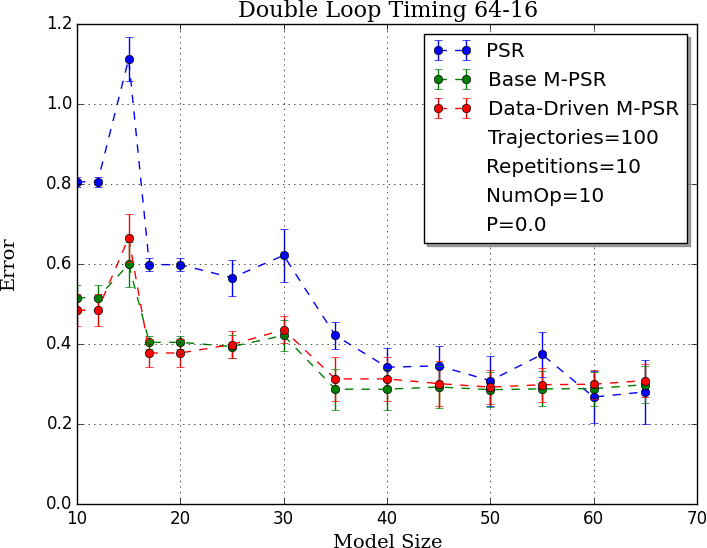
\includegraphics[width=44mm]{64-16-100.png}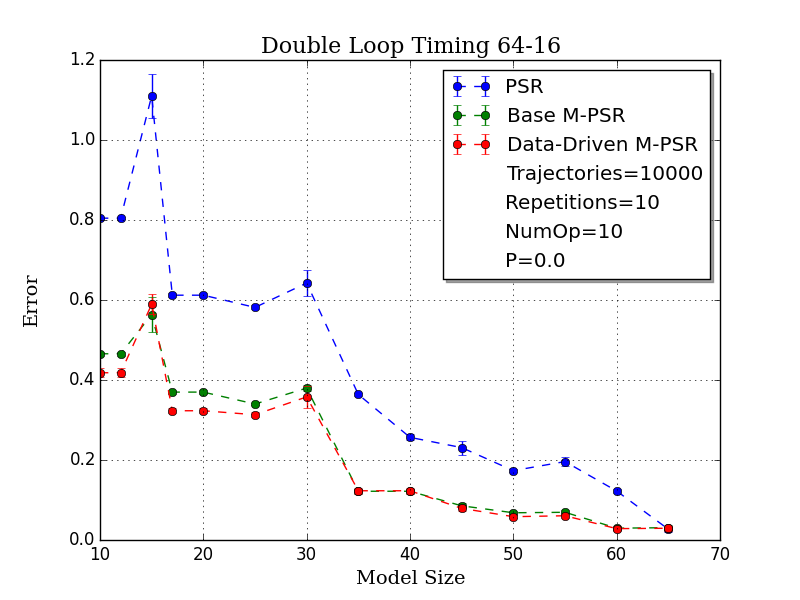
\includegraphics[width=44mm]{64-16-10000.png}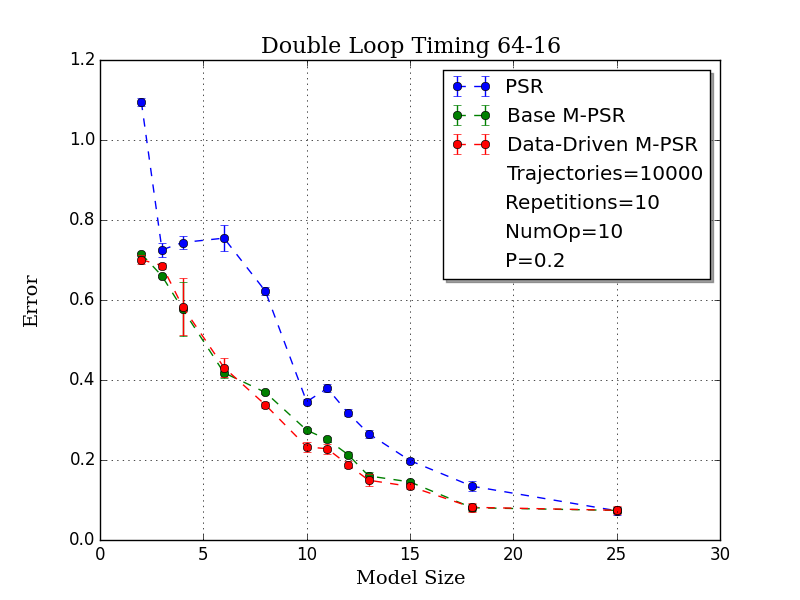
\includegraphics[width=44mm]{NoiseInfo.png}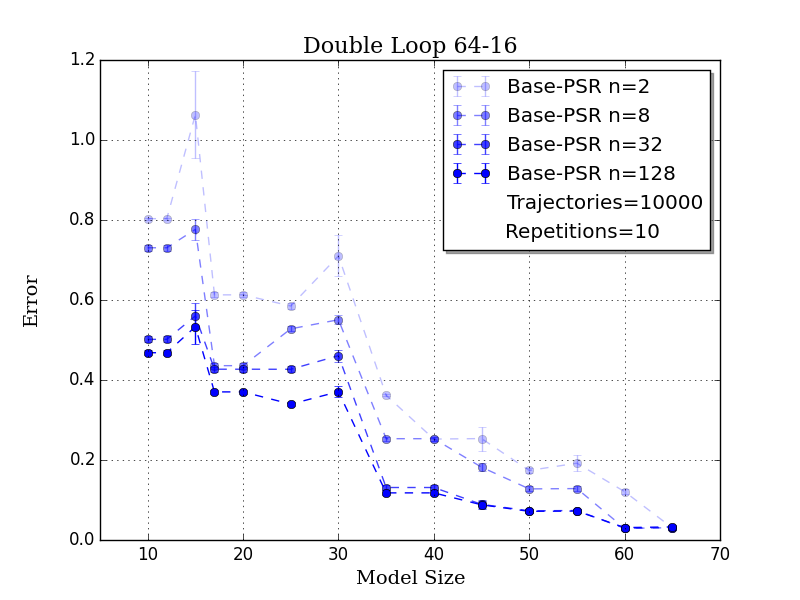
\includegraphics[width=44mm]{basePows.png}%
\vspace*{-4mm}
\caption{Results for the Double Loop of size 64-16 with (in order) a low amount of data, high amount of data and varying amount of noise (right two panels)\label{fig-double}\vspace*{-4mm}}
\end{figure*}

In this section, we assess the performance of PSRs and M-PSRs in various environments, with different model sizes, and learned from both large and small datasets. For all the plots, the x-axis is model size of the PSR/M-PSRs and the y-axis is an error measurement of the learned PSR/M-PSRs.

In all the experiments, an agent is positioned in  a partially observable environment and navigates  stochastically based on state to state transition probabilities. An observation symbol is produced on every transition. When the agent exits, we record the concatenation of the symbols produced, which represents the observation sequence.  We perform experiments in two environments: a Double Loop maze and a Pacman-style environment, depicted in Figure~\ref{overflow}.

\begin{figure}[t]
\centering
\raisebox{-0.5\height}{
\includegraphics[width=35mm]{doubleLoopImage.png}}
%\caption{Double Loop Environment\label{overflow}}
%\end{figure}
%
%\begin{figure}[ht!]
%\centering
\raisebox{-0.5\height}{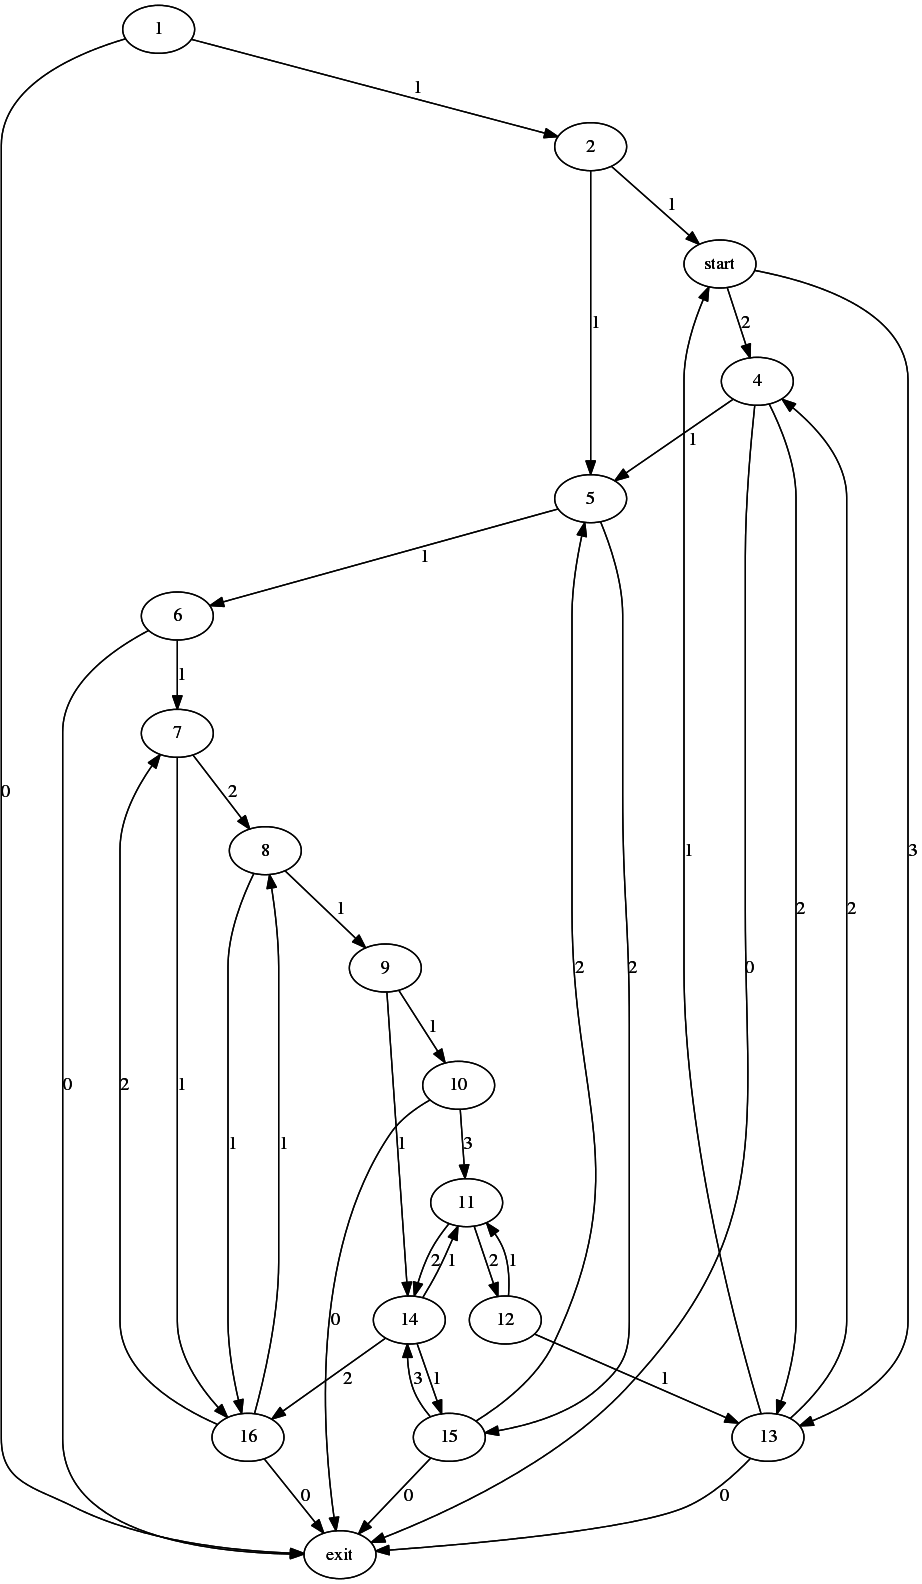
\includegraphics[width=40mm,height=50mm]{graphPacMan.png}}
%\vspace*{-4mm}
\caption{The Double Loop environment (left) and the Pacman Labyrinth (right)\label{overflow}\vspace*{-4mm}}
\end{figure}

For the Base M-PSR (i.e., the timing models), we construct the empirical Hankel matrix by taking $\Ps, \Ss = \{a^i, \forall i \leq n\}$, where $n$ is an application-dependent parameter. For Double Loop environments, we set $n = 150$, while for the Pacman domain, $n = 600$. For these choices of $n$, we verify that as the amount of data increases, the learned PSR with the true model size converges to the true model. For the Base M-PSR, we set $b=2, K=8$, so that the longest string in $\Sigma'$ is $a^{256}$.

For the tasks with multiple observations, a slightly more complex approach is required to choose $\Ps$ and $\Ss$. For the prefixes $\Ps$, we select the $k$ most frequent prefixes from our observation set. For the suffixes $\Ss$, we take all suffixes that occur in $\Ps$. We also require prefix completeness. That is, if $p'$ is a prefix of $p \in \Ps$, then $p' \in \Ps$. This heuristic for constructing empirical Hankel matrices was given in previous work~\cite{icml12}. For the Base M-PSR, we take $K=8$ and $B=2$ for both symbols $\Sigma=\{g,b\}$, where $g$ stands for green and $b$ for blue. For the Tree M-PSR, we set $L=7$ for a total of 128 operators, a far larger limit  than for the other M-PSRs. 

%\subsection{Measuring Performance}

To measure the performance of a PSR/M-PSR we use the following norm:
\begin{equation*}
\|f - \hat{f}\|_2 = \sqrt{\sum_{x \in \Sstar}(f(x) - \hat{f}(x))^2} \enspace,
\end{equation*}
where $f$ denotes the true probability distribution over observations and $\hat{f}$ denotes the function associated with the learned M-PSR/PSR. In our environments, $f$ can be computed exactly, as we have access to the underlying HMMs.

Since the set of observations $\Sigma^{\star}$ is infinite, we compute approximations to this error norm by fixing a set of strings $T$ and summing over it. For the Base M-PSR (timing) case, we take $T = \{a^i, \forall i \leq C\}$ with $C=600$. Importantly, $C$ has to be  large enough, such that $\sum_{i=0}^{C} f(a^i)>0.99$. For the multiple observation case, we take all possible strings that can be produced from the prefixes and suffixes in our dataset: $T = \{ps, \forall p \in \Ps, \forall s \in \Ss\} $

%\lucas{Need citation for bound on norm2 error}

\subsection{Double Loop Timing}

We start by considering the Double Loop environment, and the task of learning timing models. The length of a loop is the number of states in the loop. A trajectory begins with the agent at the intersection of the two loops. Here, the agent has a 50\% probability of entering either loop. At intermediate states, the agent moves to the next state in the loop with probability $1-P$ or remains in its current state with probability $P$. Exit states are located halfway into each loop. The agent leaves the environment at exit states with 50\% probability. 


\begin{figure}[ht!]
\centering
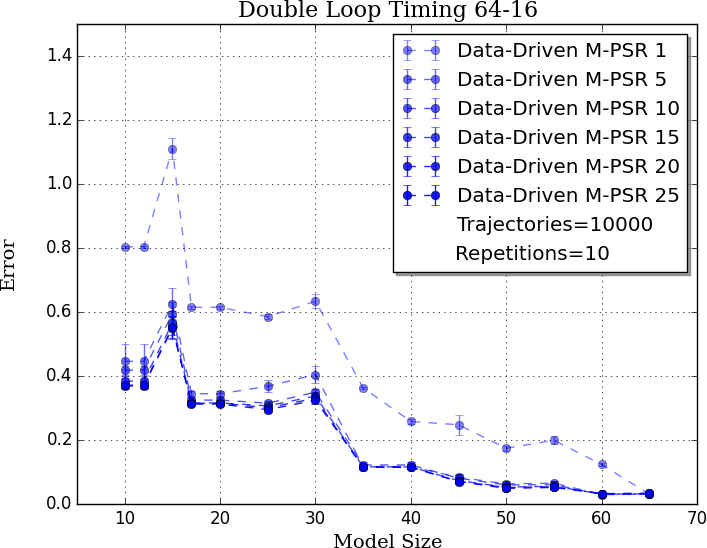
\includegraphics[width=40mm]{NumOpsTiming.png}\vspace*{-4mm}
\caption{Effect of the number of operators on performance in 64-16 loop\label{fig-numops}\vspace*{-4mm}}
\end{figure} 


%\subsection{Number of Trajectories}

Figure~\ref{fig-double} provides results for the case in which one loop consists of 64 states and the other of 16 states. The leftmost panel presents the results when learning from  100 observation sequences, while the results in the next panel are obtained using 10000 observations. In both cases, the M-PSRs  outperform the simple PSR for small model sizes. The right panels show the effect of 
varying the self-transition probability $P$, in order to to simulate noise in the environment. The two panels show curves of $P=0.2$ and $P=0$ respectively. We find that the environment with noisy loops is more compressible, that is, one can achieve better performance for low model sizes, but the performance becomes worse as the model size attains the environment's true size. M-PSRs still significantly outperform the standard PSR for reduced model sizes.  The rightmost panel also illustrates the effect of $K$ on the performance of the Base M-PSRs. We note that larger values of $K$ have better performance, up to $K=7$.

\begin{figure}[ht!]
\centering
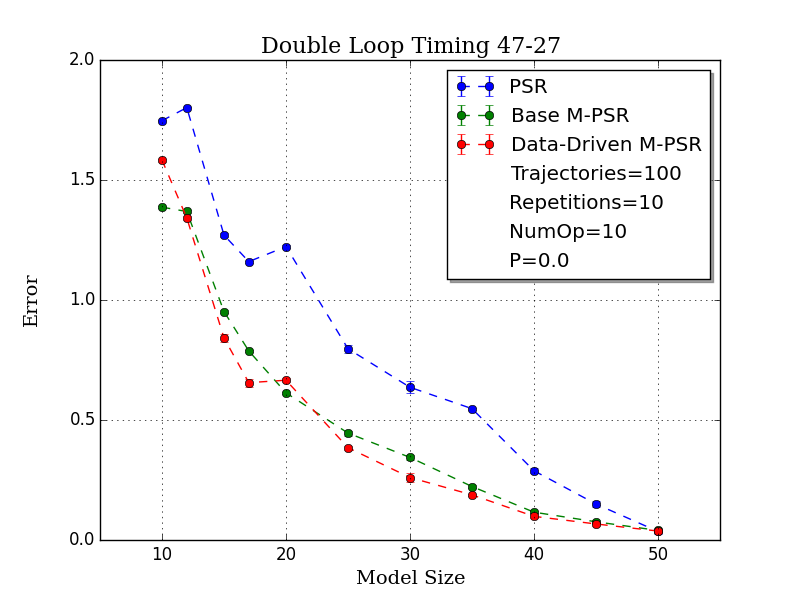
\includegraphics[width=40mm]{47-27-10000.png}\vspace*{-4mm}
\caption{High Data Double Loop 47-27\label{fig-dl47}\vspace*{-4mm}}
\end{figure}



\begin{figure*}[ht!]
%
%\begin{figure}[ht!]
%\centering
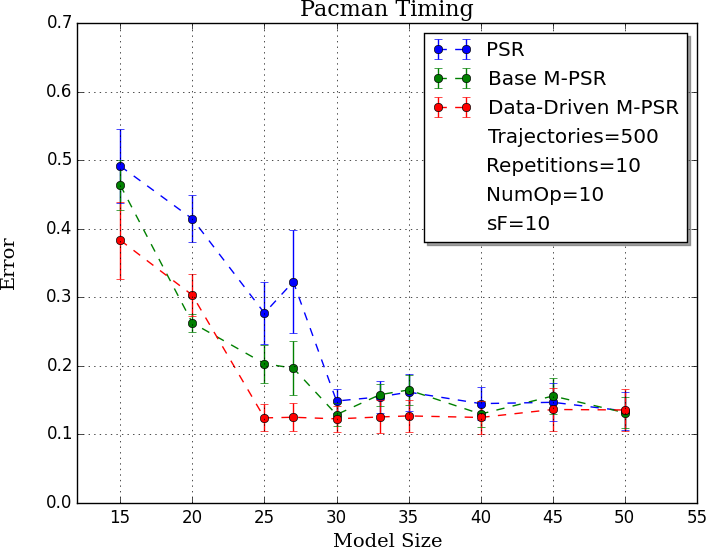
\includegraphics[width=42mm]{Pacman500.png}
%\caption{Low Data Pacman Labyrinth\label{fig-paclow}}
%\end{figure}
%
%
%\centering
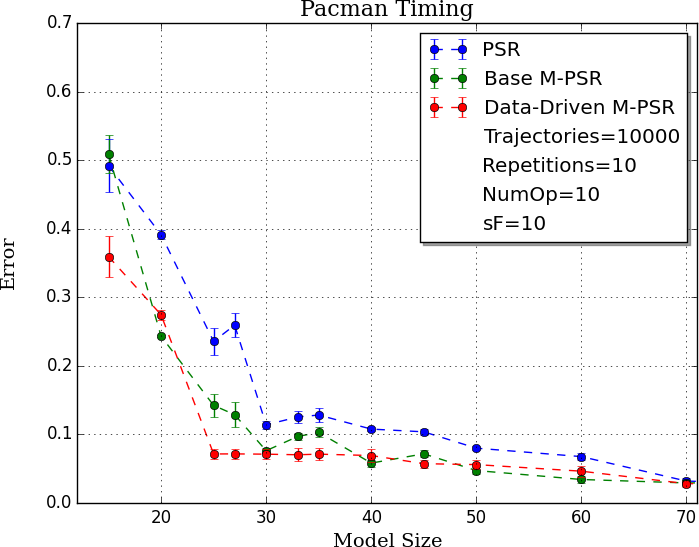
\includegraphics[width=42mm]{Pacman10k.png}
%\caption{High Data Pacman Labyrinth\label{fig-pachigh}}
%\end{figure}
%
%
%
%\begin{figure}[ht!]
%\centering
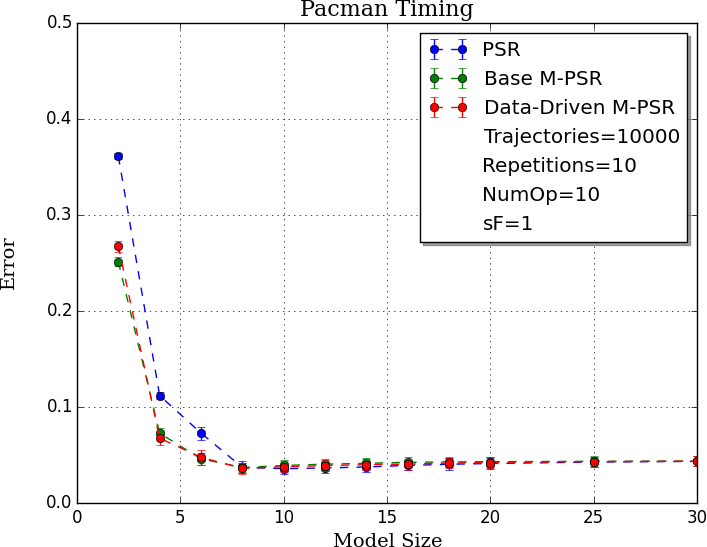
\includegraphics[width=42mm]{PacmanSF-1.png}
%\caption{Stretch Factor: 1\label{fig-pacsf1}}
%\end{figure}
%
%\begin{figure}[ht!]
%\centering
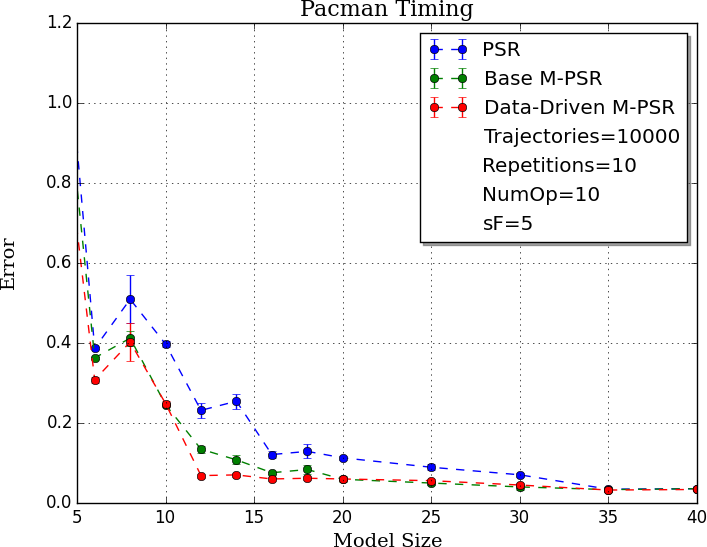
\includegraphics[width=42mm]{PacmanSF-5.png}\vspace*{-4mm}
\caption{Results for the Pacman environment with (in order from left to right) low amount of data, high amount of data and stretch factor equal to 1 and 5 (right panels)\label{fig-pacsf5}\vspace*{-4mm}}
\end{figure*}


\begin{figure*}[t!]
\centering
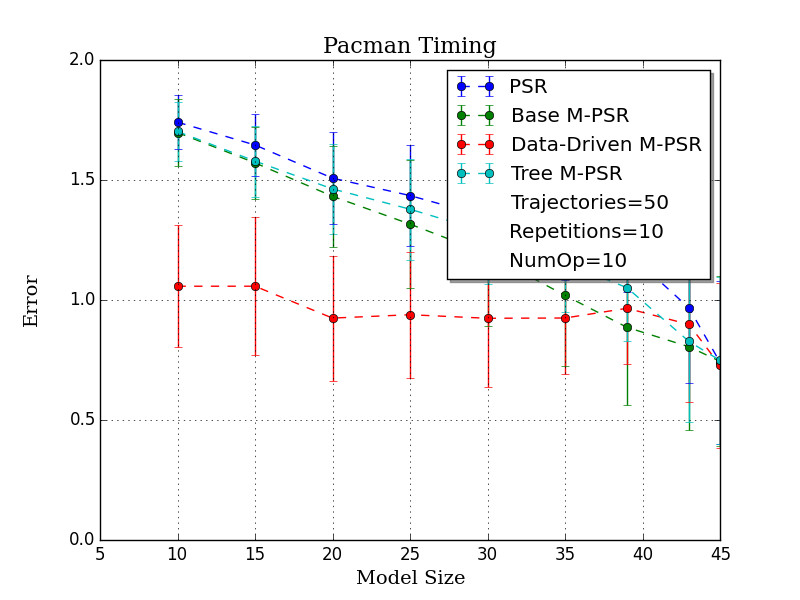
\includegraphics[width=42mm]{MO_50.png}
%\caption{Low Data Colored Loops 27-17\label{fig-collow}}
%\end{figure}
%
%\begin{figure}[ht!]
%\centering
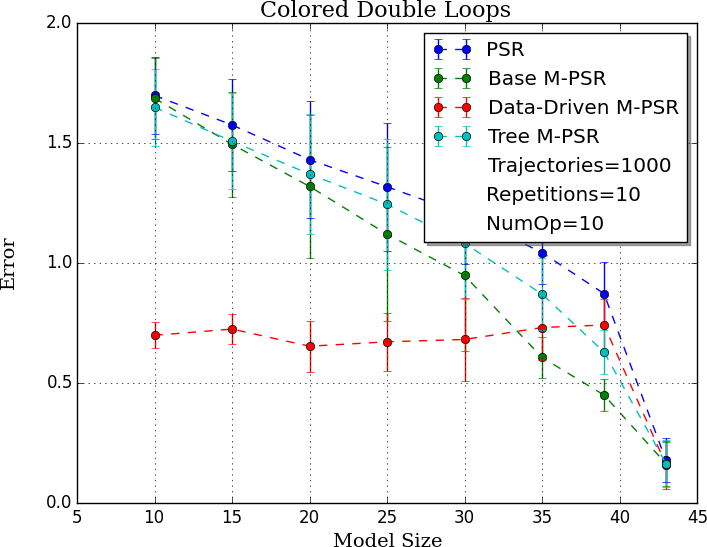
\includegraphics[width=42mm]{MO_1k.png}
%\caption{High Data Colored Loops 27-17\label{fig-colhigh}}
%\end{figure}
%
%
%
%
%\begin{figure}[ht!]
%\centering
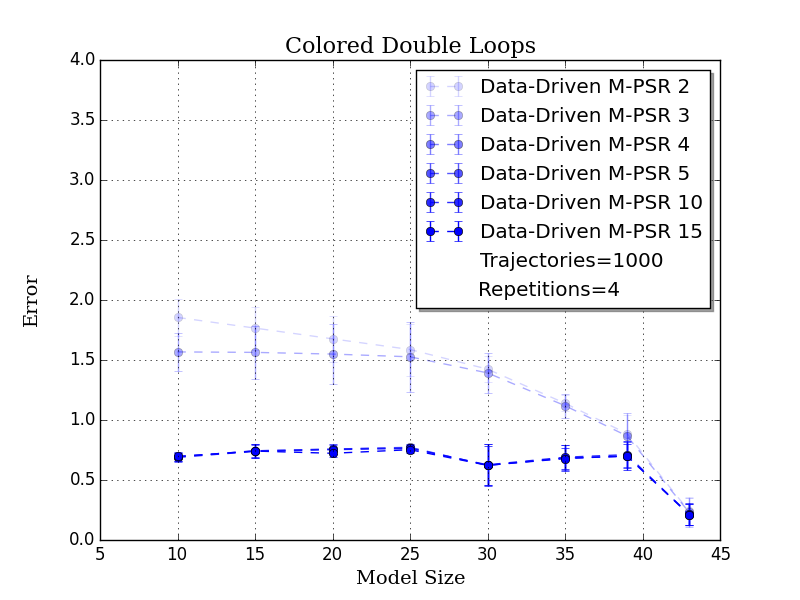
\includegraphics[width=42mm]{numOpComparison.png}\vspace*{-4mm}
\caption{Results for Coloured Double loops 27-17, in low data regime (left, high data regime (middle) and as a function of different numbers of operators (right)\label{fig-colnumops}\vspace*{-4mm}}
\end{figure*}



In Figure~\ref{fig-numops}, we illustrate how varying the number of multi-step transition operators affects performance for the 64-16 double loop. As expected, a higher number of operators improves performance, but the effect tapers off at about 20 operators. Here, the most important operators are: $\{a,a^{8},a^{24},a^{32},a^{72}\}$ which are closely tied to the environment's periodic structure.

%\subsection{Loop Lengths}

In Figure~\ref{fig-dl47}, we plot the results of a 47-27 labyrinth.  Here, because of the lengths of the loops, observations will not be as compactly expressed from the Base M-PSR. Again, M-PSRs outperform the standard PSR for reduced model sizes.



\subsection{Pacman Labyrinth Timing}


We now turn our attention to the environment on the right of Figure~\ref{overflow}. Transitions to new states occur with equal probability. The weight $w(u,v)$ between states $u$ and $v$ corresponds to the number of time steps taken to get from $u$ to $v$. We add a parameter $sF$ (stretch factor) which is used to scale all of the weights in the graph. 
In the left panels of Figure~\ref{fig-pacsf5} we vary the number of observations used for learning. M-PSRs outperform the traditional PSR regardless of the amount of data.  In the right two panels, we vary the stretch factor parameter, while  keeping the size of the dataset fixed. We find that a higher value of $sF$ provides increased improvement of the M-PSR relative to the standard PSR.

\subsection{Multiple Observations: Coloured Loops}

To test the case of multiple observations, we construct a Double Loop environment where the first loop has length $l_1=27$ and observations are green. The second loop is blue, with length $l_2=17$. We fix the length of each trajectory at 
$3 (l_1 + l_2)$
We build empirical estimates for the Hankel matrix as follows:
\begin{equation*}
%f(x)=\dfrac{count([s \in Obs, s=x])}{count([s \in Obs, |s| \geq x])} 
f(x) = \frac{|\mathrm{train} \cap x \sstar |}{|\mathrm{train} \cap \Sigma^{\geq |x|}|} \enspace.
\end{equation*}  
This means that the PSRs will compute the probability of $x$ occurring as a prefix.

As for the timing case, we vary the amount of data used to  learn the PSRS/M-PSRs in the left panels of Figure~\ref{fig-colnumops}, and we find that M-PSRs perform far better, especially the Data-Driven M-PSR. In the right panel we vary the number of multi-step transition operators learned. The important operators learned are $\{g,b,g^{27},b^{17}\}$, which is again very encouraging, as it reflects the structure of this particular environment.

\section{Discussion}

We presented an approach to leveraging multiple temporal scales in the behaviour of dynamical systems, in order to learn predictive state representations.  The proposed model, M-PSR, can be learned by adapting existing spectral approaches.  To our knowledge, the only other work that attempts to include temporal abstraction in PSRs is due to ~\cite{wolfe06}, who's use temporally extended actions, or options~\cite{sutton99}, and build PSRs on top of these.  However, this model has a very different flavour from our approach, as we bundle together observations into multiple steps.  In particular, our approach is applicable even when there are no actions, such as in the case of HMMs, whereas this previous work requires structure in the action space.
In all the experiments we conducted, M-PSRs offer significantly better predictive performance for reduced model sizes than PSRs. In addition, Data-Driven PSRs offer improvements over generic M-PSRs by learning the transition operators specific to the environment, which is very important when prior information about appropriate time scales for modelling is not known.  Our evaluation focused on illustrating the advantage of the proposed model especially when the amount of data available is small, and in noisy environments.
 Although this was not specifically illustrated in the experiments. M-PSRs offer a computational advantage when performing conditional probability queries as they use far fewer matrices than regular PSRs. This can be very important for online applications, such as in planning environments. 
 
 We presented a comprehensive set of experiments in simulated domains, in order to have some ground truth available.  However, we anticipate that the proposed models would be useful in real tasks, for example in financial market prediction.  In this case, one could discretize market levels into bins, and use M-PSRs to learn predictive models over multiple time steps, in order to capture both long-term trends and fast fluctuations.  We also plan to experiment with this approach in the domain of processing physiological signal recordings, which similarly exhibit short and long-term trends.  On the theoretical side, it would be interesting to analyze the existence of an ``optimal" set of symbols for the data-driven M-PSR, and to develop further algorithms for finding it.

\section*{Acknowledgments}
SOME FUNDING?

\bibliographystyle{named}
\bibliography{references}

\end{document}

